\documentclass[tikz,border=10pt]{standalone}
\usepackage{tikz-3dplot}
\usepackage{amsmath, amssymb}
\usetikzlibrary{arrows.meta, positioning, calc, decorations.pathreplacing, 3d}
\usetikzlibrary{matrix, fit, backgrounds, shapes}
\usetikzlibrary{angles,quotes}

\usepackage[T1]{fontenc}
\usepackage[utf8]{inputenc}
\usepackage{newpxtext,newpxmath}
\usepackage{sectsty}

\begin{document}
%========================================================
% TikZ #2 (Step 2): define reflection in {u,v}-coordinates
%========================================================	
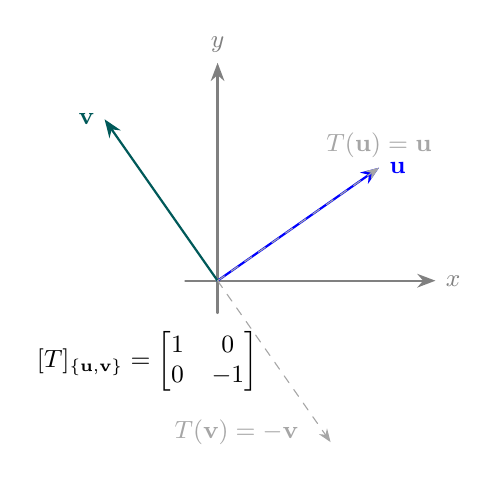
\begin{tikzpicture}[scale=2.05, >=Stealth, line cap=round, line join=round]
	\def\m{0.7}
	
	\pgfmathsetmacro{\ux}{1}
	\pgfmathsetmacro{\uy}{\m}
	\pgfmathsetmacro{\vxB}{-\m}
	\pgfmathsetmacro{\vyB}{1}
	
	\tikzset{
		axis/.style={thick, gray},
		uvec/.style={thick, blue},
		vvec/.style={thick, teal!70!black},
		help/.style={dashed, gray!70},
		box/.style={rounded corners, draw=gray!60, fill=white, inner sep=3pt},
		mat/.style={font=\small}
	}
	
	\newcommand{\panelaxes}{
		\draw[axis,->] (-0.2,0) -- (1.35,0) node[right] {\small $x$};
		\draw[axis,->] (0,-0.2) -- (0,1.35) node[above] {\small $y$};
	}
	
%	\node[box, anchor=west] at (-1.5,-1.38) {\small Step 2: define reflection in the new coordinates};
	
	\panelaxes
	
	\draw[uvec,->] (0,0) -- (\ux,\uy) node[pos=1, right] {\small $\textbf{u}$};
	\draw[vvec,->] (0,0) -- (\vxB,\vyB) node[pos=1, left]  {\small $\textbf{v}$};
	
	\draw[help,->] (0,0) -- (\ux,\uy) node[pos=1, above] {\small $T(\textbf{u})=\textbf{u}$};
	\draw[help,->] (0,0) -- ({-\vxB},{-\vyB}) node[pos=0.80, below left] {\small $T(\textbf{v})=-\textbf{v}$};
	
	\node[anchor=west, mat] at (-1.18,-.5)
	{$[T]_{\{\textbf{u},\textbf{v}\}}=\begin{bmatrix}1&0\\0&-1\end{bmatrix}$};
	
\end{tikzpicture}
\end{document}